\documentclass[11pt,openany]{memoir}
\usepackage[usenames,dvipsnames]{xcolor}
\usepackage{amssymb}
\usepackage{amsmath}
\usepackage{amsthm}
\usepackage{url}
\usepackage{xspace}
\usepackage[margin=2.5cm]{geometry}
\usepackage{tikz}
\usetikzlibrary{positioning,calc,matrix,arrows}
\usepackage{pgfplots}
\usepackage{listings}
\usepackage{color}
\usepackage{textcomp}
\usepackage{fancyvrb}
\usepackage{array}
\usepackage{dirtytalk}
\usepackage[colorlinks]{hyperref}
\usepackage{cleveref}

% NOTE: This template is based on the MatConvNet manual written by Andrea Vedaldi, Karel Lenc and Ankush Gupta.

\newtheorem{example}{Example}
\newtheorem{lemma}{Lemma}

\newcommand{\real}{\mathbb{R}}
\newcommand{\xx}{\mathbf{x}}
\newcommand{\yy}{\mathbf{y}}
\newcommand{\pp}{\mathbf{p}}
\newcommand{\hh}{\mathbf{h}}
\newcommand{\diag}{\operatorname{diag}}
\newcommand{\bone}{\mathbf{1}}
\newcommand{\FF}{\mathcal{F}}
\newcommand{\ththeta}{\pmb{\theta}}
\newcommand{\EE}{\mathbb{E}}
\DeclareMathOperator{\dd}{\text{d}}
\newcommand{\vv}{\operatorname{vec}}
\newcommand{\tr}{\operatorname{tr}}
%\newcommand{\matconvnet}{\textsc{MatConvNet}\xspace}
%\newcommand{\matlab}{\textsc{MATLAB}\xspace}
%\newcommand{\cpp}{C{}\texttt{++}~}
%\newcommand{\by}{\mathbf{y}}
%\newcommand{\bc}{\mathbf{c}}
%\newcommand{\bz}{\mathbf{z}}
%\newcommand{\bff}{\mathbf{f}}
%\newcommand{\bg}{\mathbf{g}}
%\newcommand{\br}{\mathbf{r}}
%\newcommand{\bw}{\mathbf{w}}
%\newcommand{\bp}{\mathbf{p}}
%\newcommand{\bfs}{\mathbf{s}}
%\newcommand{\bfe}{\mathbf{e}}
\newcommand{\samsays}[1]{\textcolor{RubineRed}{[S: #1]}}

%\newcommand{\argmin}{\operatornamewithlimits{argmin}}
%\newcommand{\argmax}{\operatornamewithlimits{argmax}}
%\newcommand{\sign}{\operatornamewithlimits{sign}}
%
%\tikzstyle{block} = [draw, rectangle, minimum height=3em, minimum width=3em]
%\tikzstyle{data} = []
%\tikzstyle{datac} = [draw, circle, minimum height=2.5em, minimum width=2.5em,inner sep=3pt,font=\footnotesize]
%\tikzstyle{par} = [draw, circle, minimum height=2.5em, minimum width=2.5em,fill=black!20,inner sep=3pt,font=\footnotesize]
%\tikzstyle{pinstyle} = [pin edge={to-,thin,black}]
%\tikzstyle{to} = [->,>=stealth',shorten >=1pt,semithick]
%\tikzstyle{from} = [<-,>=stealth',shorten >=1pt,semithick]
%\tikzstyle{bp} = [draw=blue,text=blue]
%\tikzstyle{bpl} = [draw=blue!40]
%\tikzstyle{bpe} = [text=blue,draw=none]

\VerbatimFootnotes

\setsecnumdepth{subsection}
\settocdepth{subsection}

\definecolor{listinggray}{gray}{0.9}
\definecolor{lbcolor}{rgb}{0.8,0.8,0.8}
\lstset{
	%backgroundcolor=\color{lbcolor},
	tabsize=4,
	rulecolor=,
	language=matlab,
	basicstyle=\small,
	upquote=true,
	columns=fullflexible,
	showstringspaces=false,
	extendedchars=true,
	breaklines=false,
	prebreak = \raisebox{0ex}[0ex][0ex]{\ensuremath{\hookleftarrow}},
	%frame=single,
	showtabs=false,
	showspaces=false,
	showstringspaces=false,
	identifierstyle=\ttfamily,
	keywordstyle=\color[rgb]{0,0,1},
	commentstyle=\itshape\color[rgb]{0.133,0.545,0.133},
	stringstyle=\color[rgb]{0.627,0.126,0.941},
}
\lstMakeShortInline[columns=fullflexible, breaklines = true,
 breakatwhitespace = true]!

\title{Old Ideas for Applied Computer Vision}
\author{
Samuel Albanie
}
\date{}

\hypersetup{
  pdfinfo={
    Title={Classics/Kernels for Applied Computer Vision},
    Author={Samuel Albanie},
		Subject={Notes on Mathematics},
    Keywords={computer vision, differentials, machine learning}
  }
}

\sloppy

% ------------------------------------------------------------------
\begin{document}
% ------------------------------------------------------------------

%\end{document}

\frontmatter
\maketitle{}

\begin{abstract}
This note is designed to gather together information about some of the work that has gone on over the last few decades of computer vision research.
The goal is to develop it over time and therefore it should be considered a work-in-progress.  Consequently any contributions, feedback or notifications of mistakes are much appreciated\footnote{Feel free to contact me by raising an issue on the github page, submitting a pull request directly (\mbox{\url{https://github.com/albanie/derivations})}}).
\end{abstract}
\clearpage

\tableofcontents*
\clearpage

\mainmatter
\chapter{Introduction}\label{sec:intro}

Calculus plays a central role in computer vision. As the community has integrated ever more closely with techniques from machine learning, statistics and optimisation, the ability to differentiate vector and matrix functions has become more useful to computer vision researchers.  Unfortunately, multivariate calculus, when performed with indices over element locations is a fairly tricky business to build an intuition for.  Although the index-based approach has the majority of the market share in the research world, there is an alternative: the slightly lesser known method of \textit{matrix differentials}.  We have found this alternative approach to be significantly simpler, more intuitive and faster to work with.  

Finally, we note that the widespread adoption of automatic differentiation (autodiff) has been a major boon to the whole community, in many cases obviating the need to perform arduous pen and paper derivations.  The goal of these notes is not to encourage the reader to avoid using autodiff, but to assist them in understanding, on a mathematical level, what is going on \say{under the hood}.


\section{Useful Resources}

There are a number of extremely good references for getting to grips with the calculus of vector and matrix functions.  Below are a few that we have found particularly useful, providing much of the material for these notes:

\begin{itemize}
\item Written by econometricians Magnus and Neudecker (originally in $1988$, but revised several times), \textit{Matrix differential calculus with applications in statistics and econometrics} is the canonical reference for matrix differential calculus~\cite{magnus1988matrix}.
\item The fundamentals of working with matrices \cite{searle2017matrix}.
\item \cite{kinghorn1996integrals}, \cite{minka2000old} and \cite{petersen2008matrix} each contain a large number of highly useful results and are good as quick references.
\item The MatConvNet manual \cite{vedaldi2015matconvnetmanual} provides carefully worked through examples of matrix derivatives.  While the emphasis is primarily on index-based derivations, it provides the derivatives of many common neural network computation blocks in matrix form and is very useful as a reference. 
\end{itemize}
\chapter{Scale Space} \label{chap:scale-space}

One of the fundamental challenges in building systems that can understand images is the construction of good \textit{representations}.  Since even a relatively small image comprises a vast quantity of data, we would like to distill the information down to a much more compact form that tells us about the things we care about in the image and is \textit{invariant} to things we don't care about.  

Early work focused on simple representations of an image, such as the extrema in the signal (e.g. edges, dots etc.) and their first or second derivatives - a line sketch can contain much of the semantic content of an image while requiring far fewer bits of information to store.  However, this approach quickly runs into difficulties.  Over what scale should the derivatives of the image signal be taken?  Edges which define important for objects at one scale, such as the grains on a piece of wood, are irrelevant at another scale, such as a picture of a forrest. 

There have been several major contributions in this area, but perhaps the most important was the introduction of \textit{scale space filtering} \cite{witkin1987scale}.  The core idea is that the image should be represented simultaneously by a set of multiple scales.  This is achieved by simply convolving the source image with Gaussian filters of increasing bandwidth (this is illustrated with a one dimensional signal in Fig.~\ref{fig:scales}).  

\begin{figure}
\centering
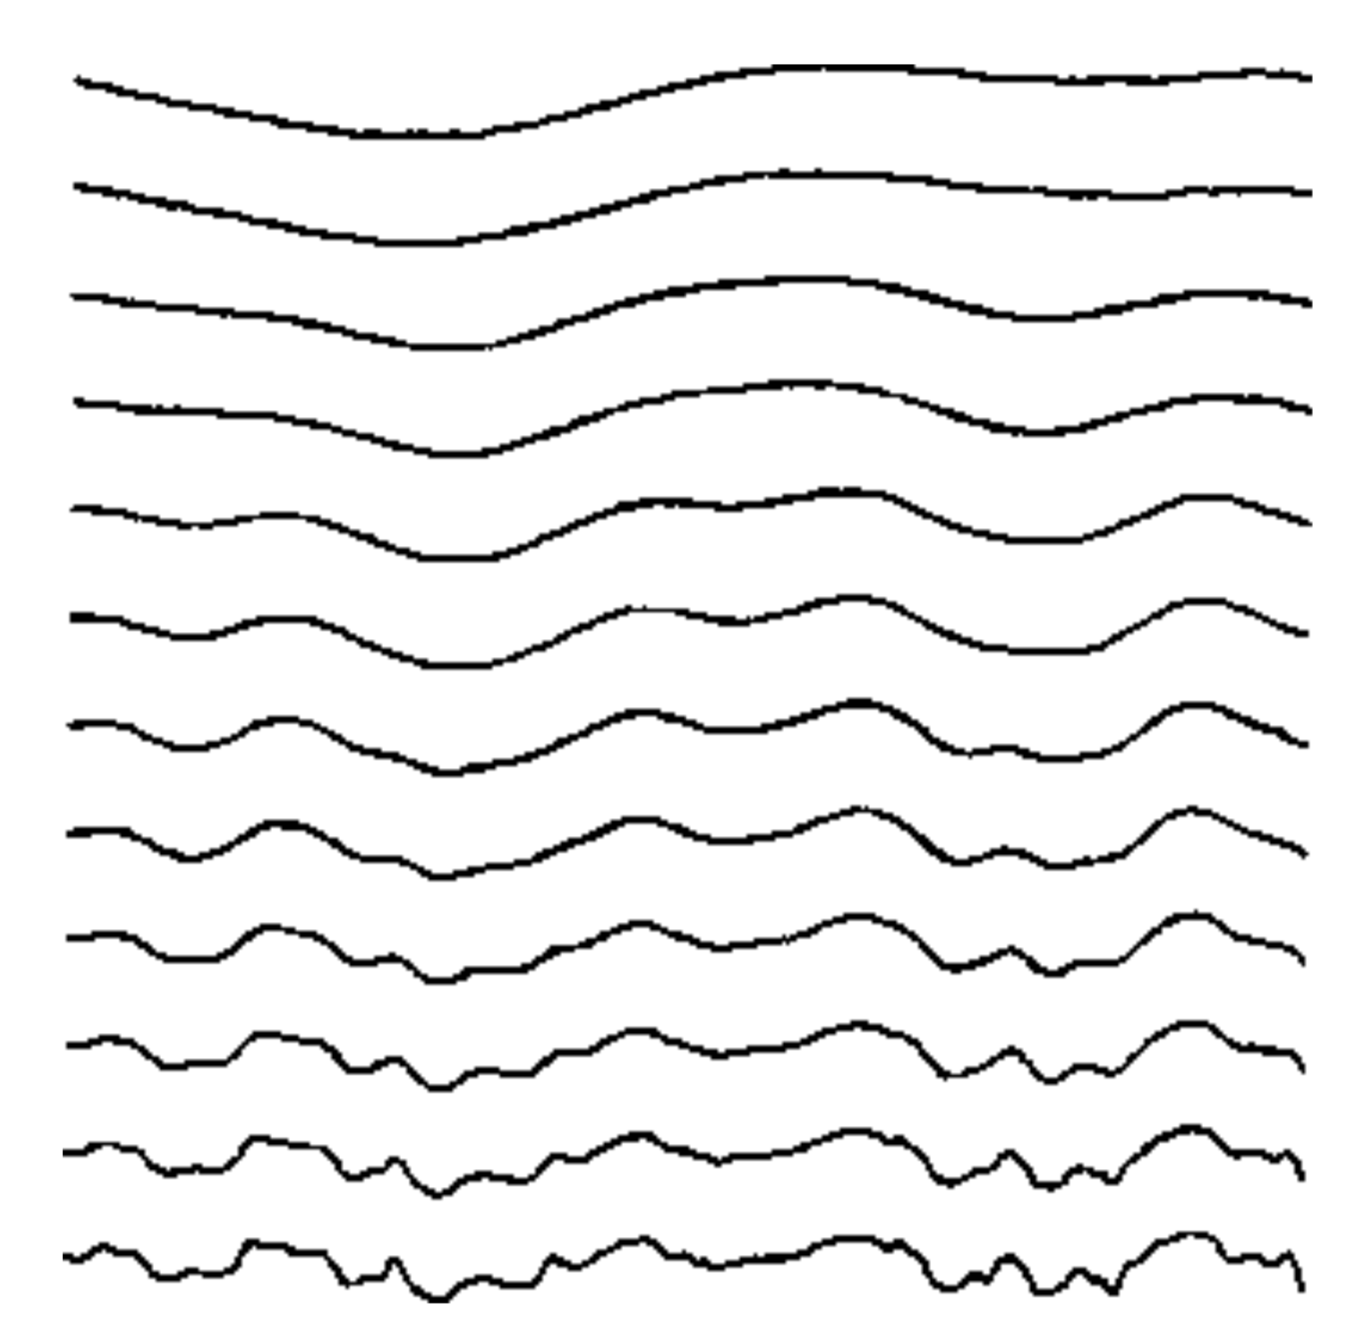
\includegraphics[height=0.3\textwidth]{figs/scale-space.png}
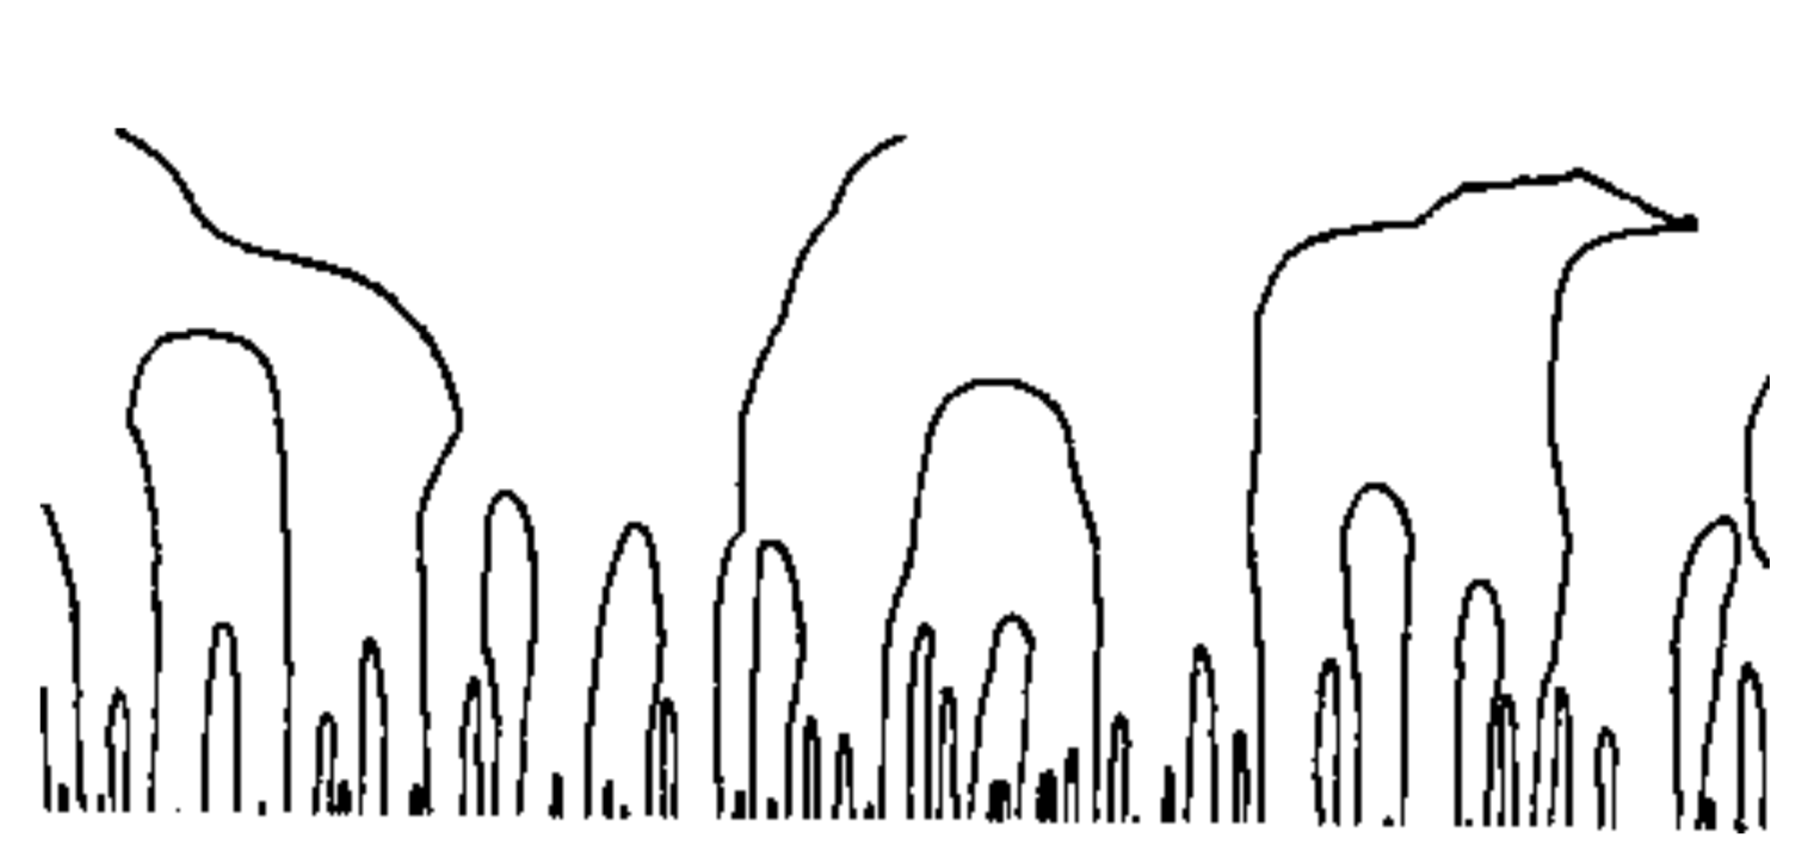
\includegraphics[height=0.25\textwidth]{figs/zero-crossings.png}
\caption{\textbf{Left}: The scale space of a one-dimensional signal $\phi$.  At the bottom is the raw signal, which has been smoothed by Gaussian kernels with increasing bandwidth as you move up the figure. \textbf{Right:} The level sets $ \phi_{xx} = $ corresponding to the scale space shown on the left.  In both images the $x$-axis is horizontal and the vertical axis represents the value fo $\sigma$ (the bandwidth of the smoothing kernel). These figures originally appeared in \cite{witkin1987scale}).\label{fig:scales}}
\end{figure}

In the original work, Witkin focused on using the zeros of the second derivative (i.e. the inflection points) of the signal as the representation

% ------------------------------------------------------------------
\bibliographystyle{plain}
\bibliography{../bib/refs.bib}
\end{document}
% ------------------------------------------------------------------

